\documentclass[notitlepage,cs4size,punct,oneside]{ctexrep}

% default paper settings, change it according to your word
\usepackage[a4paper,hmargin={2.54cm,2.54cm},vmargin={3.17cm,3.17cm}]{geometry}

\usepackage{amsmath,amssymb,amsthm}
\usepackage{titlesec}

% 公式编号的计数格式, 在章内计数
\numberwithin{equation}{chapter}

% set the abstract format, need abstract package

\usepackage[runin]{abstract}
\usepackage{algorithm}
\usepackage{algpseudocode}
\usepackage{booktabs}
\usepackage{graphicx}
\usepackage{float} % 图片和表格定位
\usepackage{subfigure} % 子图包
\usepackage{xcolor}




\usepackage[pdfborder={0 0 0},colorlinks=true,linkcolor=blue,CJKbookmarks=true, unicode=true]{hyperref}
%若要用LATEX编译, 请用下面的命令替代上述命令:
% \usepackage[dvipdfm,pdfborder={0 0 0},colorlinks=true,linkcolor=blue,CJKbookmarks=true]{hyperref}

\usepackage{mathrsfs}
\usepackage{longtable}

%\usepackage{boondox-calo}
%\usepackage{dutchcal}

\setlength{\absleftindent}{1.5cm} \setlength{\absrightindent}{1.5cm}
\setlength{\abstitleskip}{-\parindent}
\setlength{\absparindent}{0cm}

% Theorem style
\newtheoremstyle{mystyle}{3pt}{3pt}{\kaishu}{0cm}{\bfseries}{}{1em}{}
\theoremstyle{mystyle}

\newtheorem{definition}{\hspace{2em}定义}[chapter]
% 如果没有章, 只有节, 把上面的[chapter]改成[section]
\newtheorem{theorem}[definition]{\hspace{2em}定理}
\newtheorem{axiom}[definition]{\hspace{2em}公理}
\newtheorem{lemma}[definition]{\hspace{2em}引理}
\newtheorem{proposition}[definition]{\hspace{2em}命题}
\newtheorem{corollary}[definition]{\hspace{2em}推论}
\newtheorem{remark}{\hspace{2em}注}[chapter]
%类似地定义其他“题头“. 这里“注“的编号与定义、定理等是分开的

\def\theequation{\arabic{chapter}.\arabic{equation}}
\def\thedefinition{\arabic{chapter}.\arabic{definition}.}

% title - \zihao{1} for size requirement \bfseries for font family requirement
\title{{\zihao{1}\bfseries 期中作业:微调与目标检测}}

\author{何益涵 \quad 20307110032\\吕文韬 \quad }

\date{}
%%%%%%%%%%%%%%%%%%%导言区设置完毕
%%%%%%%%%%%%%%%%%%%%%%%%%%%%%%%%%%%%%%%%%%%%%%%%%%%%%%%%%%%%%%%%%%%%%
\begin{document}
%Styles for chapters/section
%若要将章标题左对齐, 用下面这个语句替换相应的设置
%\CTEXsetup[nameformat={\raggedright\zihao{3}\bfseries},%
\CTEXsetup[nameformat={\zihao{3}\bfseries},
           format={\zihao{3}\bfseries\centering},
           beforeskip={0.8cm}, afterskip={1.2cm}]{chapter}
\CTEXsetup[nameformat={\zihao{4}\bfseries},
           format={\zihao{4}\bfseries\centering},
           name={第~,~节},number={\arabic{section}},
           beforeskip={0.4cm},afterskip={0.4cm}]{section}
\CTEXsetup[nameformat={\zihao{-4}\bfseries},
           format={\zihao{-4}\bfseries},
           number={\arabic{section}.\arabic{subsection}.},
           beforeskip={0.4cm},afterskip={0.4cm}]{subsection}
\CTEXoptions[abstractname={摘要: }]
\CTEXoptions[bibname={\bfseries 参考文献}]

\renewcommand{\thepage}{\roman{page}}
\setcounter{page}{1}
% \tableofcontents\clearpage

\maketitle\renewcommand{\thepage}{\arabic{page}}
\thispagestyle{empty}\setcounter{page}{0}
%%%  论文的页码从正文开始计数, 摘要页不显示页码
% 撰写论文的摘要
\renewcommand{\abstractname}{摘要: }
\begin{abstract}
     本项目的仓库地址为:

     \url{https://github.com/HeDesertFox/Neural-Networks-and-Deep-Learning-Homework-Group-Tasks.git}。

     详见其中的文件夹\texttt{group\_task2}。其中包含微调任务\texttt{task1\_finetuning}和目标检测任务\texttt{task2\_object\_detection}。

     本项目提供了训练好的模型,详见\texttt{task1\_finetuning}中的\texttt{model\_pretrained\_state\_dict.pth}和\texttt{model\_random\_state\_dict.pth}文件,以及\texttt{task2\_object\_detection}中的。。。文件。也可以点击以下网盘链接:。。。\\



\end{abstract}



\chapter{微调在ImageNet上预训练的卷积神经网络实现鸟类识别}
\section{任务描述}
\begin{enumerate}
\item 修改现有的CNN架构(如AlexNet,ResNet-18)用于鸟类识别,通过将其输出层大小设置为200以适应数据集中的类别数量,其余层使用在ImageNet上预训练得到的网络参数进行初始化;
\item 在[CUB-200-2011]数据集上从零开始训练新的输出层,并对其余参数使用较小的学习率进行微调;
\item 观察不同的超参数,如训练步数、学习率,及其不同组合带来的影响,并尽可能提升模型性能;
\item 与仅使用CUB-200-2011数据集从随机初始化的网络参数开始训练得到的结果进行对比,观察预训练带来的提升。
\end{enumerate}

\section{项目架构}
此任务的所有文件在\texttt{task1\_finetuning}文件夹中,其中包含以下文件:
\begin{enumerate}
\item \texttt{data\_loading\_preprocessing.py}文件:包含数据下载函数与预处理函数。
\item \texttt{model.py}文件:包含网络构造函数。
\item \texttt{training\_fine\_tuning.py}文件:包含训练和超参数调优函数。
\item \texttt{main\_notebook.ipynb}文件:包含微调任务的全部流程,如数据加载、调参和训练可视化。
\end{enumerate}

\section{实验设置}
\subsection{数据增广}
本实验根据CUB-200-2011中的\texttt{train\_test\_split.txt}文件对数据集进行划分,形成训练集和验证集。在数据预处理中,对训练集的数据进行了图像增强,其中包括了随机水平翻转和随机旋转。

\subsection{模型选择}
此项目的模型构建函数可以生成两种 CNN 架构:Alexnet 和 ResNet-18,并且可以选择采用Imagenet预训练的参数初始化或随机初始化。生成的模型的最后一层被替换为输出维数为200的全连接层以适应本任务的要求。

为了实现更高的模型性能,本实验采用 ResNet-18 架构,使用者可以在模型构造函数中输入参数\texttt{"alexnet"}将模型改为 Alexnet。

\subsection{优化器设置}
本实验的优化器均选择 SGD 优化器,在所有实验中都采用0.9的动量以加速收敛,采用1e-3的权重衰退缓解过拟合。

在后续的调参和训练过程中,预训练模型的学习率在最后一层都正常设置,其余层的学习率都除$10$。


\section{调参结果}
本实验调节两个参数以尽可能提高模型性能:学习率(\texttt{lr})和训练轮数(\texttt{epoch})。

总体来说,增加训练轮数不会减少验证集上的准确率。这是因为 ResNet-18 的表现力足够强,一般可以在训练集上将精度提升到接近$100\%$,此时梯度几乎为零,因此最终验证集精度不会因为训练过久而下降。

经过若干次调参,预训练模型的最后一次调参的参数列表定为 \texttt{lr}: \{0.5e-3, 1e-3, 2e-3\}, \texttt{epoch}: 20。最优参数为 \texttt{lr} = 2e-3,\texttt{epoch} = 20。

实验表明,在这三种学习率之下,精度都比较接近,略高于$70\%$,其中\texttt{lr} = 2e-3时的表现略好。

\begin{figure}[H]
    \centering
    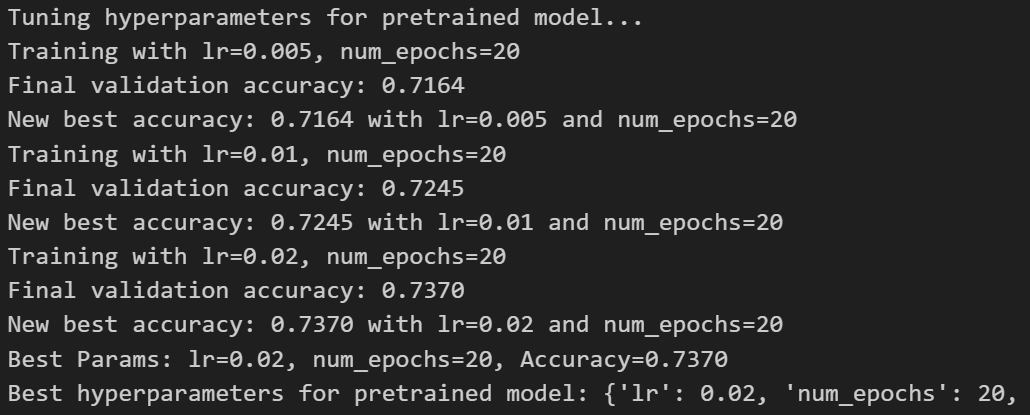
\includegraphics[scale=0.7]{fine.png}
    \caption{最后一次调参结果}
    \label{fig:fine}
\end{figure}

随机初始化模型也可以做调参。本实验中随机初始化模型采用和预训练模型一样的参数,保证比较的公平性。



\section{实验结果}
\subsection{数据分析}
以下图片中,\textcolor{orange}{橙线}都是\textcolor{orange}{预训练模型}的数据曲线,\textcolor{blue}{蓝线}都是\textcolor{blue}{随机初始化模型}的数据曲线。完整的数据文件在文件夹\texttt{run}中。

\begin{figure}[H]
    \centering
    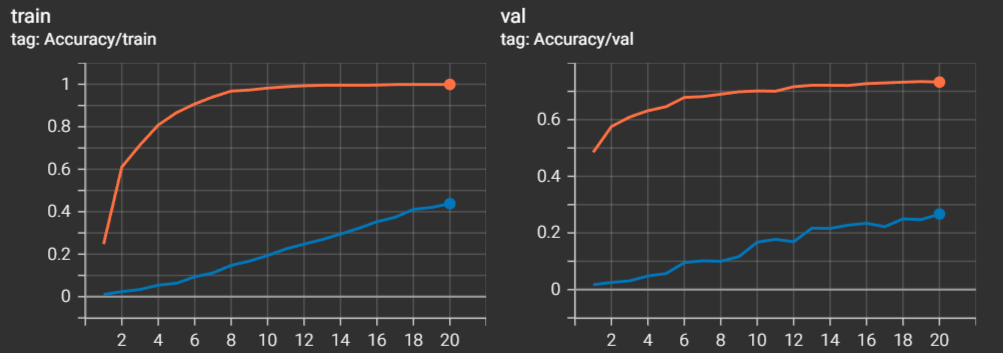
\includegraphics[scale=0.75]{acc.png}
    \caption{准确率对比}
    \label{fig:acc}
\end{figure}

预训练模型的训练准确率迅速上升,并且在初期就已经接近$1$,这表明模型能够很好地学习训练数据。准确率接近1通常表明模型对训练数据的拟合非常好。随机初始化模型的训练准确率相比之下增长较慢,最终也没有接近$1$,这可能意味着模型学习较慢,或者是模型容量不足以完全学习数据。

预训练模型的验证准确率也很快上升并保持在较高水平,这说明预训练模型在未见数据上也具有很好的泛化能力。验证准确率的高稳定性同时也表明模型没有出现显著的过拟合。随机初始化模型的验证准确率虽有所提高,但整体上显著低于预训练模型,这表明其泛化能力较弱。验证准确率的较低水平也表明该模型可能受限于其初始参数设置,未能充分利用训练数据。


\begin{figure}[H]
    \centering
    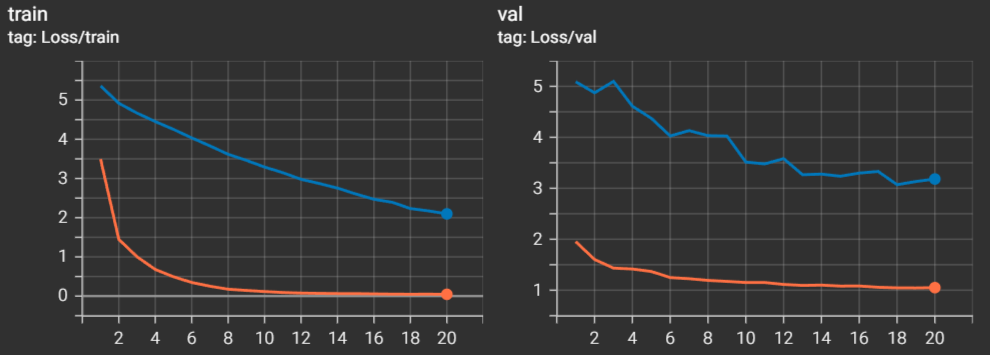
\includegraphics[scale=0.75]{loss.png}
    \caption{损失函数对比}
    \label{fig:loss}
\end{figure}

预训练模型的训练损失迅速下降并趋于平稳,这与高训练准确率一致,表明模型有效地减少了误差。随机初始化模型的训练损失下降较慢,结束时仍高于预训练模型的损失,这进一步证实了其学习效率较低。

预训练模型的验证损失下降并保持较低,与高的验证准确率相符,说明模型在未见数据上的表现良好。验证损失的低水平和稳定性表明没有过拟合。随机初始化模型的验证损失相比之下较高并稍有波动,可能指示模型在未见数据上的性能不够稳定,这可能是由于模型参数初始化不佳或者模型结构不够优化。

\subsection{结论}
预训练模型明显优于随机初始化模型,无论是在训练过程还是在验证过程中。这表明利用预训练的权重可以显著提升模型的学习效率和泛化能力。

随机初始化模型可能需要更多的训练周期、更复杂的网络结构或者更多的调优来提高其性能。

基于以上分析,使用预训练模型在类似的任务中是一个有效的策略,特别是当可用的训练数据量不足以从头训练一个复杂模型时。对于随机初始化的模型,可能需要探索额外的技术,如更深的网络、正则化策略或更精细的超参数调整,以提高其性能。



\chapter{在VOC数据集上训练并测试目标检测模型Faster R-CNN和YOLO V3}
\section{任务描述}
\begin{enumerate}
    \item 学习使用现成的目标检测框架——如mmdetection或detectron2——在VOC数据集上训练并测试目标检测模型Faster R-CNN和YOLO V3;
    \item 挑选4张测试集中的图像,通过可视化对比训练好的Faster R-CNN第一阶段产生的proposal box和最终的预测结果。
    \item 搜集三张不在VOC数据集内包含有VOC中类别物体的图像,分别可视化并比较两个在VOC数据集上训练好的模型在这三张图片上的检测结果(展示bounding box、类别标签和得分)
\end{enumerate}



\end{document}
